\documentclass[aspectratio=169]{beamer}
\usetheme{default}
\usepackage{graphicx}

\title{Implementation of a Phylogenetic Tree in Legume Information Systems (LIS)}
\author{Rishab Pradeep; Alan Cleary (Mentor)}
\institute[ICR]{Institute for Computing in Research}
\date{August 3, 2023}
\begin{document}
\begin{frame}[plain]
    \maketitle
\end{frame}
\begin{frame}
	\large{\textbf{Introduction}}
\end{frame}
\begin{frame}{What is LIS?}

	\begin{figure}
		\centering
		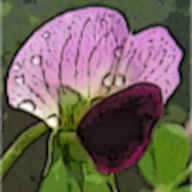
\includegraphics[width=0.2\linewidth]{imgs/lis-logo.png}
	\end{figure}
 \begin{figure}
     \centering
     
\includegraphics[width=0.2\linewidth]{imgs/ncgr-logo.png}
    
 \end{figure}
 \begin{figure}
     \centering
     
\includegraphics[height=0.3\linewidth]{imgs/usda-logo.png}
     \caption{Enter Caption}
 \end{figure}
	
\end{frame}
\begin{frame}{What is a Phylotree?}
	\begin{figure}
		\centering
		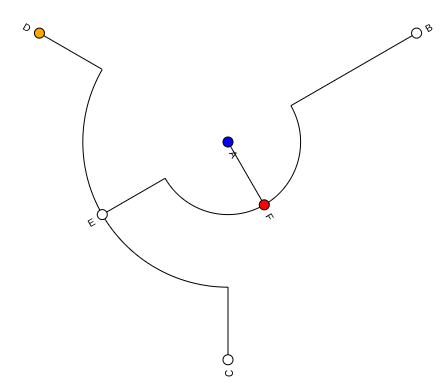
\includegraphics[width=0.55\linewidth]{imgs/phylotee}
		\caption{Sample Tree}
	\end{figure}
\end{frame}
\begin{frame}{The Scope}
	\begin{itemize}
		\item<1->LIS is almost 20 years old
		\item<2->Has underwent many iterations
		\item<3->Transition to web components
	\end{itemize}
	\end{frame}
	\begin{frame}
		\large{\textbf{Let's build a Phylotree web component}}
		\begin{figure}
			\centering
			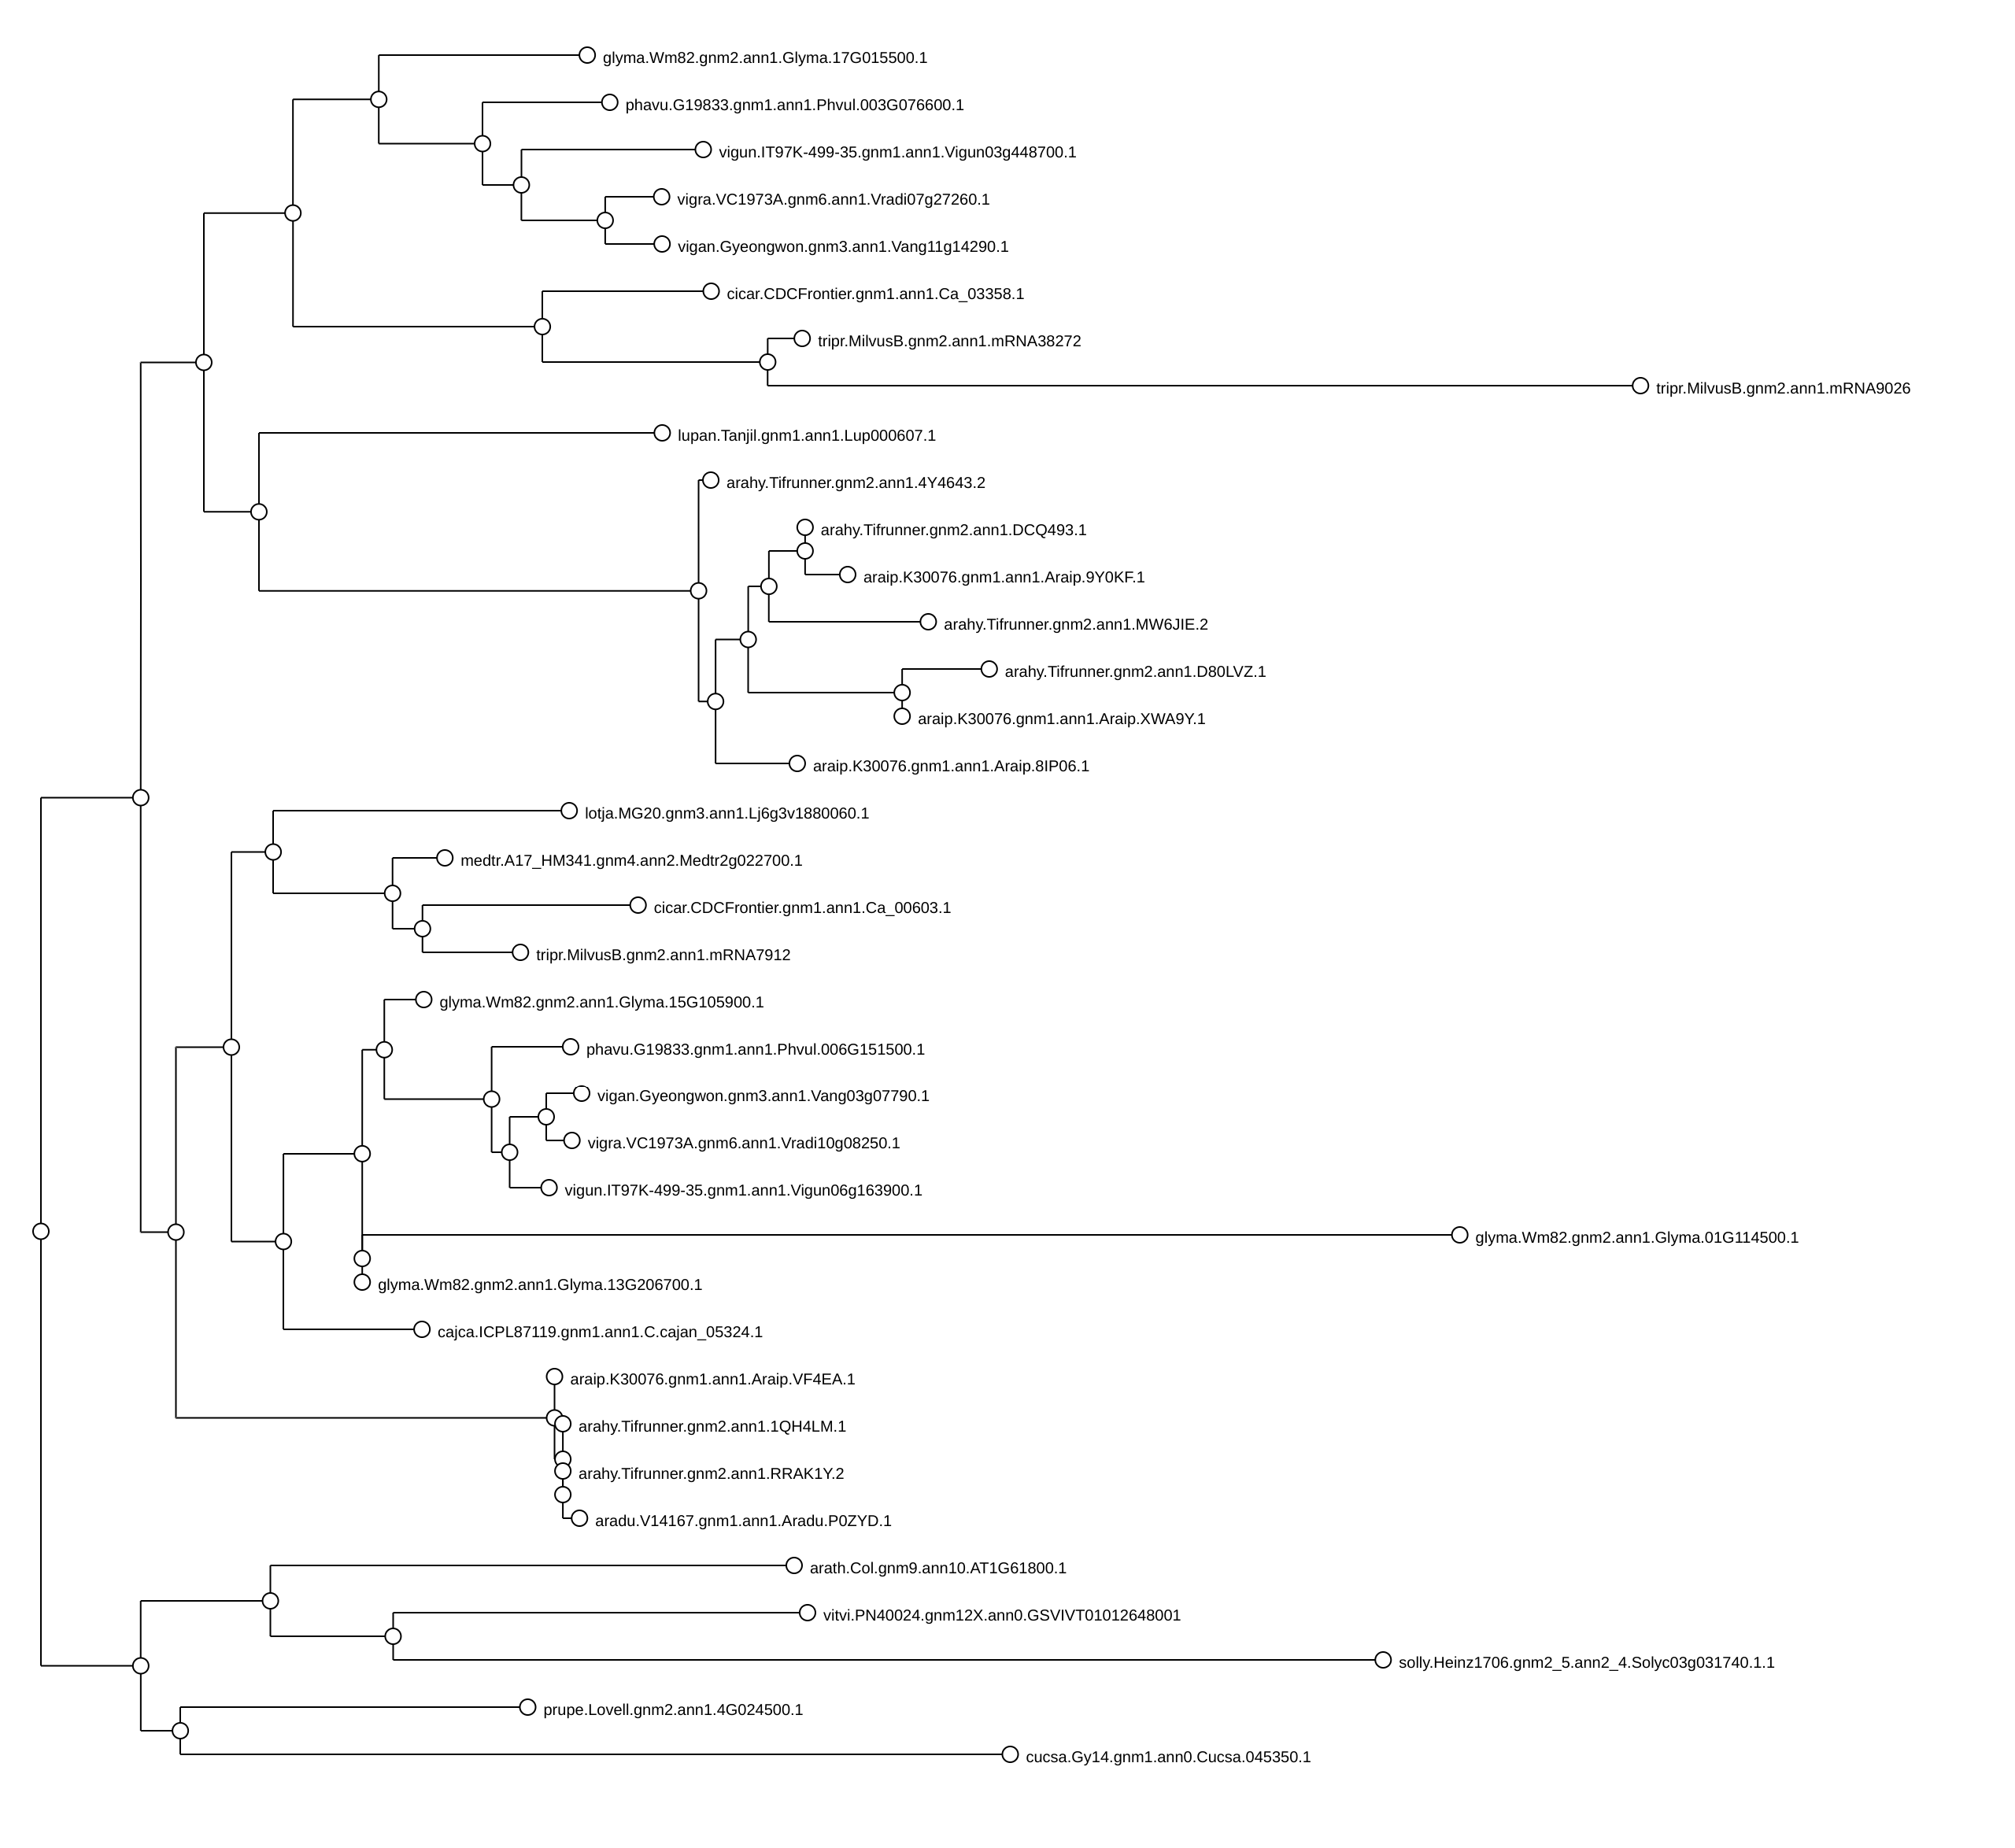
\includegraphics[height=0.5\linewidth]{imgs/black-and-white-lis-vertical-tree.png}
			\caption{Phylotree generated from Newick data pulled from LIS}
		\end{figure}	\end{frame}
	
	\begin{frame}
		\large{\textbf{The Nitty Gritty}}
		\end{frame}
		\begin{frame}{Programming}
			\only<1-> {
				\begin{figure}
					
\includegraphics[height=0.2\linewidth]{imgs/typescript-logo.png}
				\end{figure}
			}
			\only<2-> {
				\begin{figure}
					
\includegraphics[height=0.2\linewidth]{imgs/lit-logo.png}
				\end{figure}
			}
		\end{frame}
		
		\begin{frame}{The component}
			\begin{figure}
			\centering
			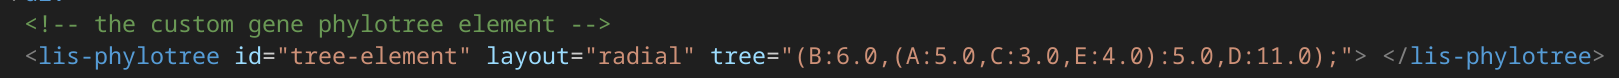
\includegraphics[width=0.7\linewidth]{imgs/web-component-call.png}
		\end{figure}
  \begin{figure}
			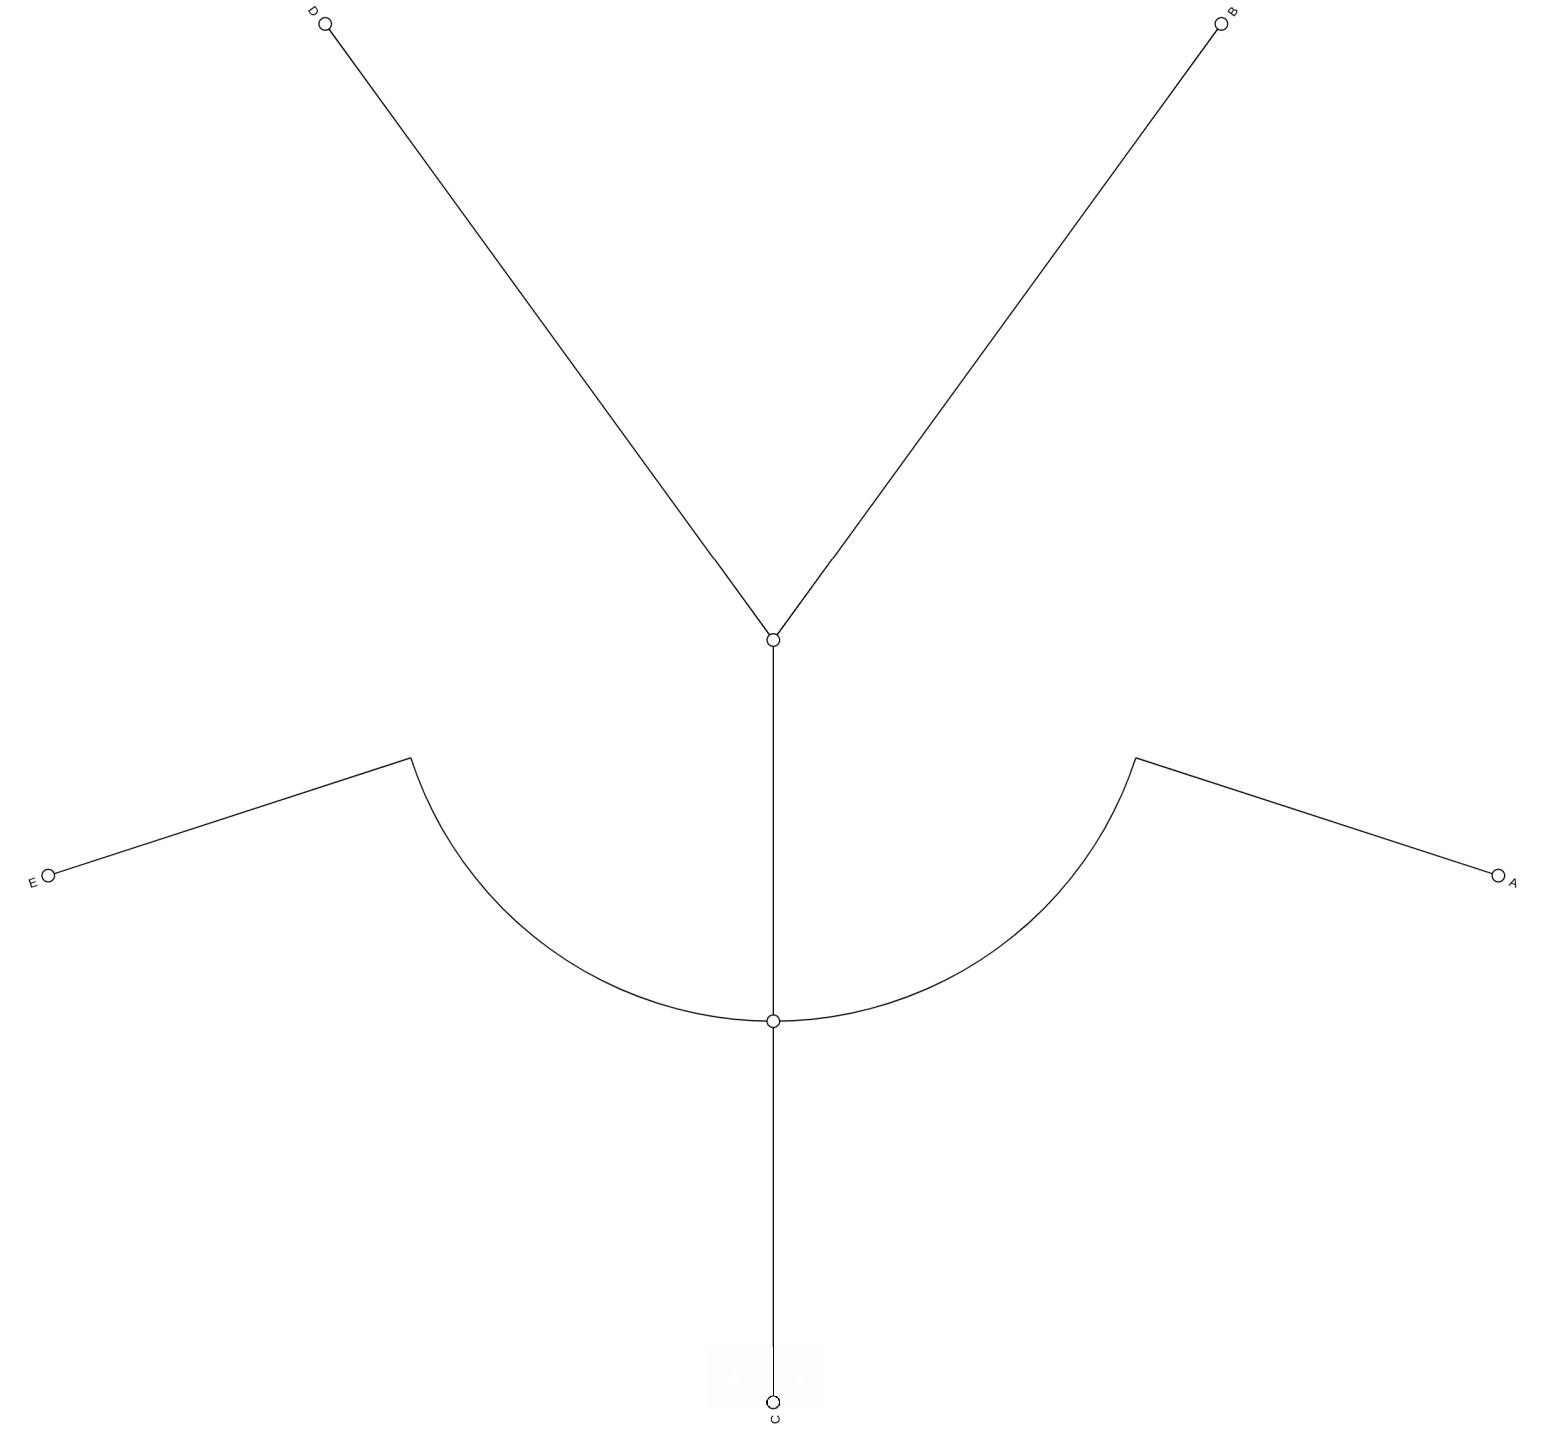
\includegraphics[height=0.4\linewidth]{imgs/radial-sample.png}
			\caption{Web component tree generated with newick input}
			\end{figure}
  \end{frame}
  \begin{frame}{How newick works}
  \begin{figure}
      \centering
      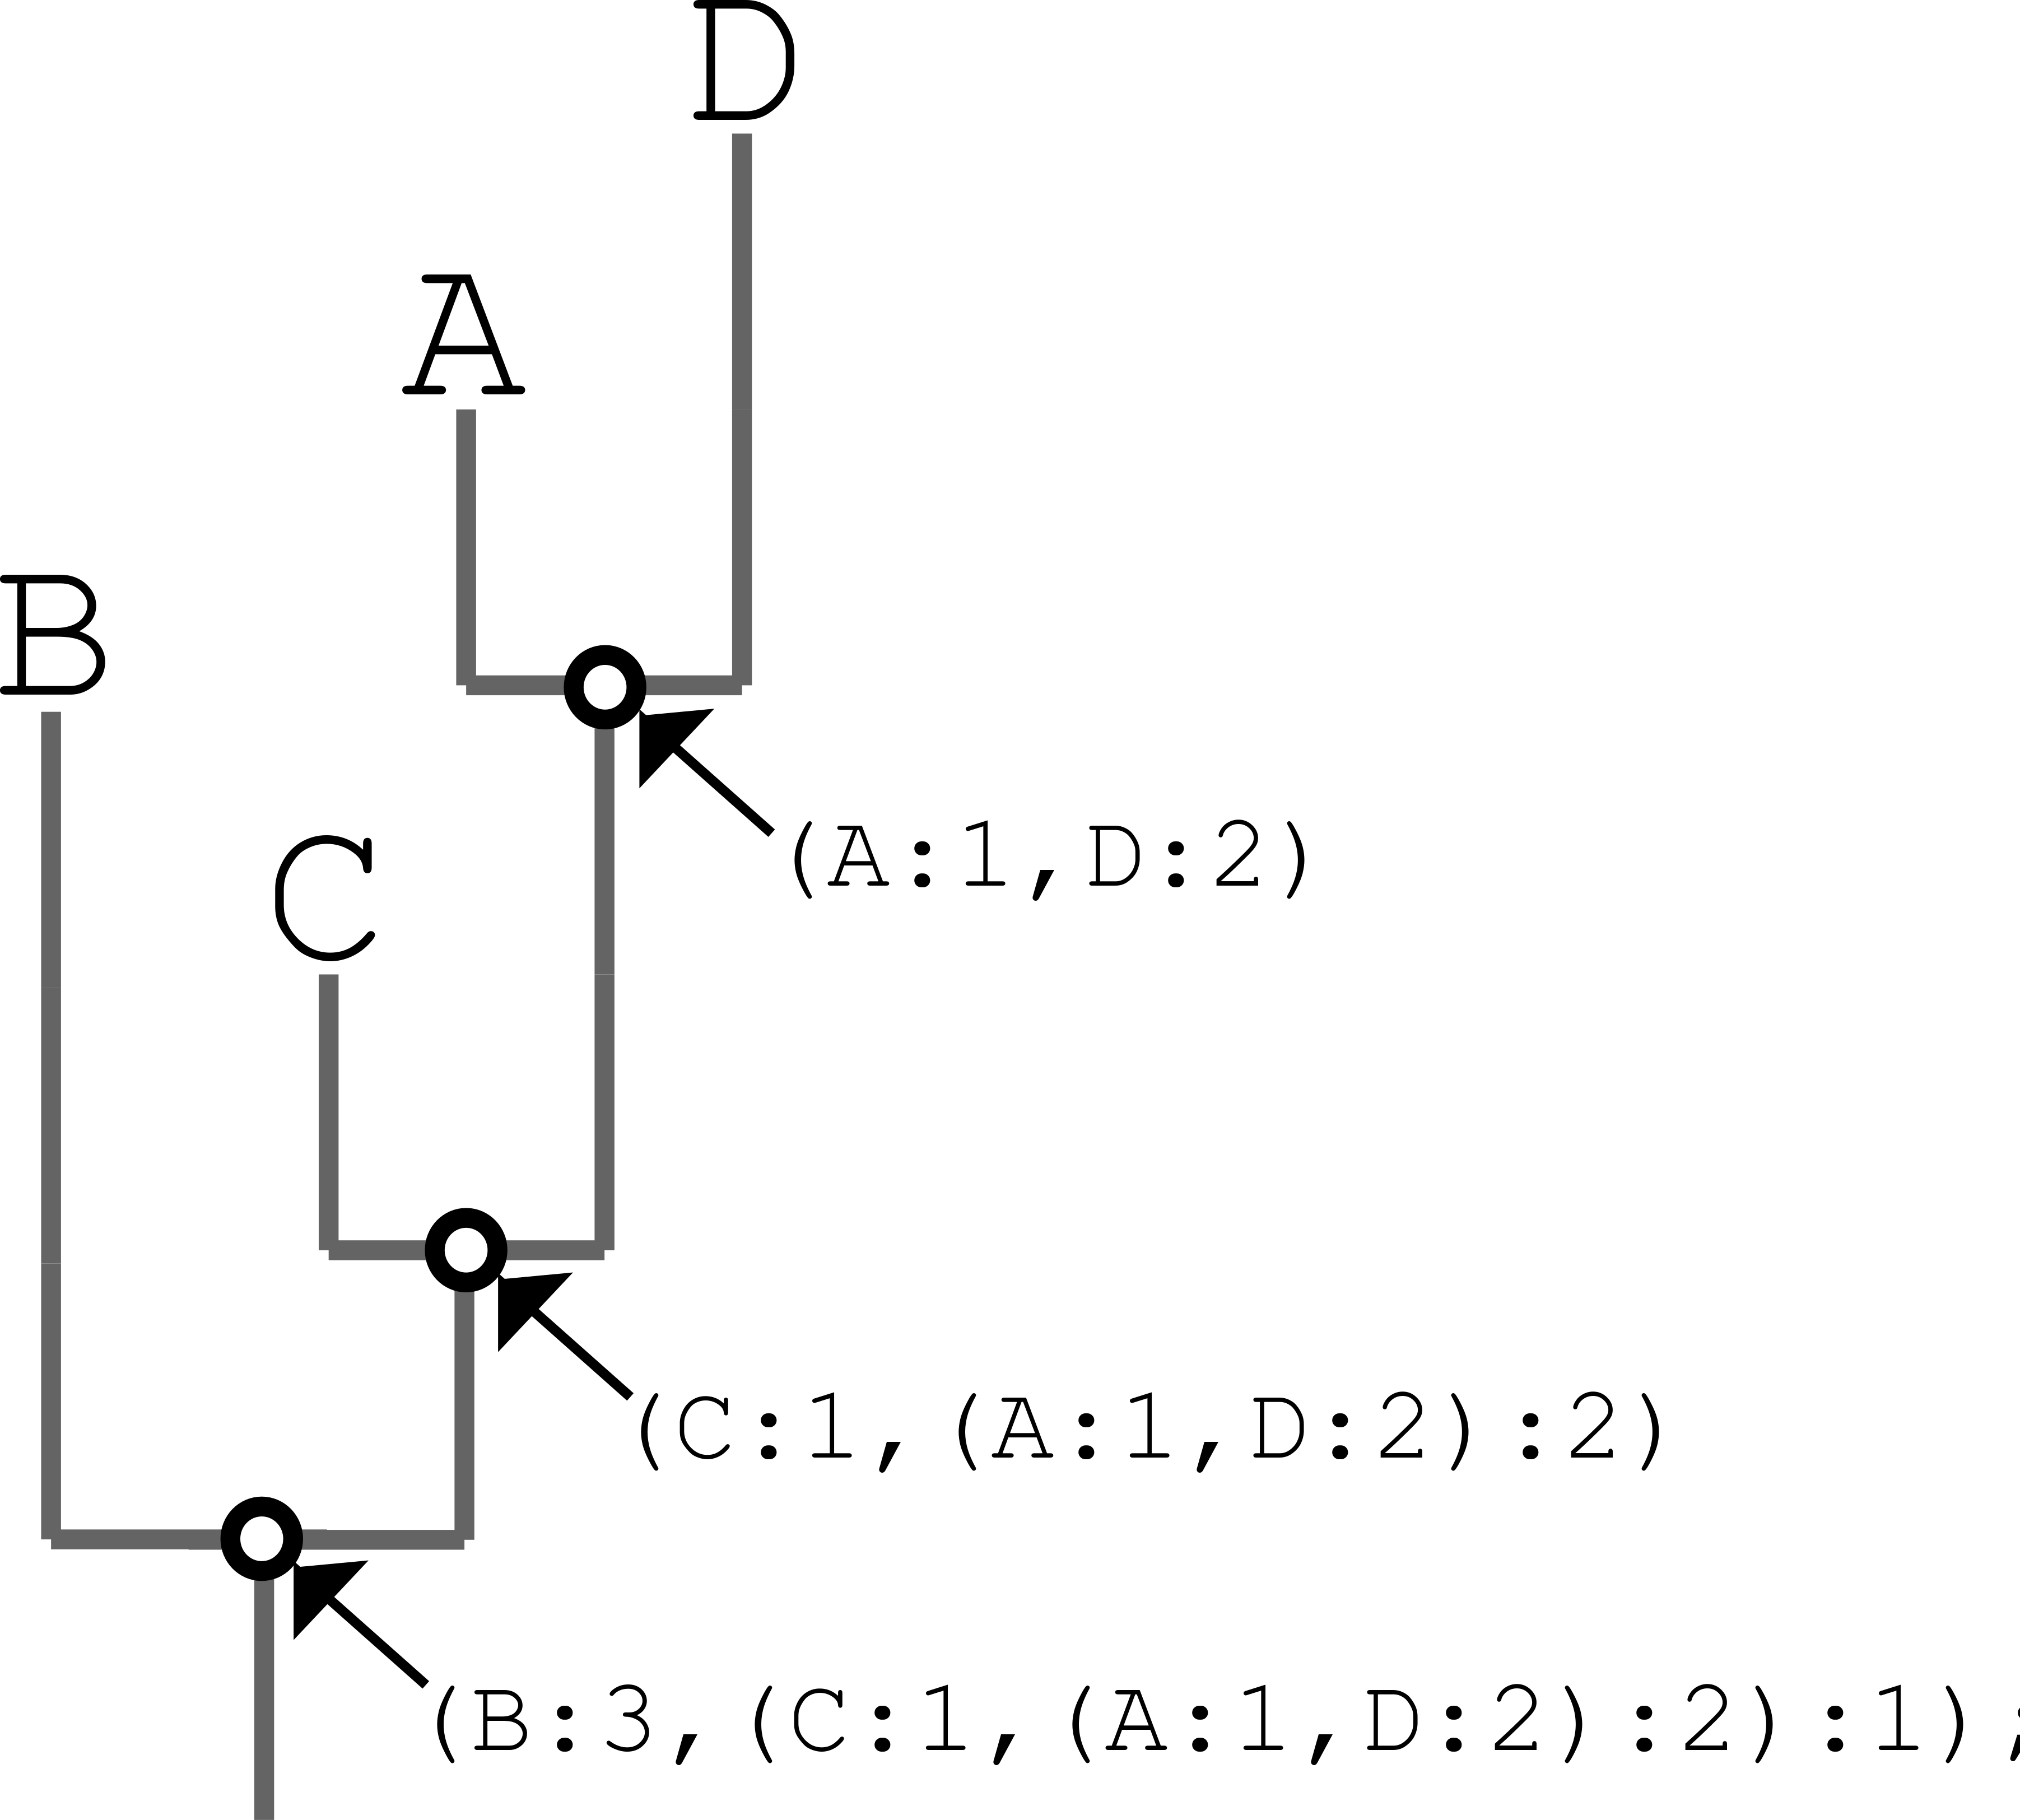
\includegraphics[width=0.5\linewidth]{imgs/newick-tree.png}
      \caption{Diagram of Newick}
      
  \end{figure}
		
			\end{frame}
			
		\begin{frame}{Structure of the Phylotree Type}
			\begin{figure}
				\centering
				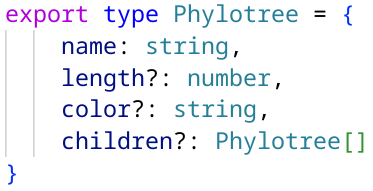
\includegraphics[width=0.7\linewidth]{imgs/phylotree-type.png}
				\caption{Phylotree type}
			\end{figure}
			\end{frame}
			\begin{frame}{Pulling data from LIS}
				\begin{figure}
					\centering
					
\includegraphics[height=0.5\linewidth]{imgs/graphql-logo.png}
					\caption{GraphQL Logo}
				\end{figure}
			\end{frame}
		\begin{frame}
			\large{\textbf{Results}}
		\end{frame}
		\begin{frame}{Results}
			\begin{figure}
			    \centering
			    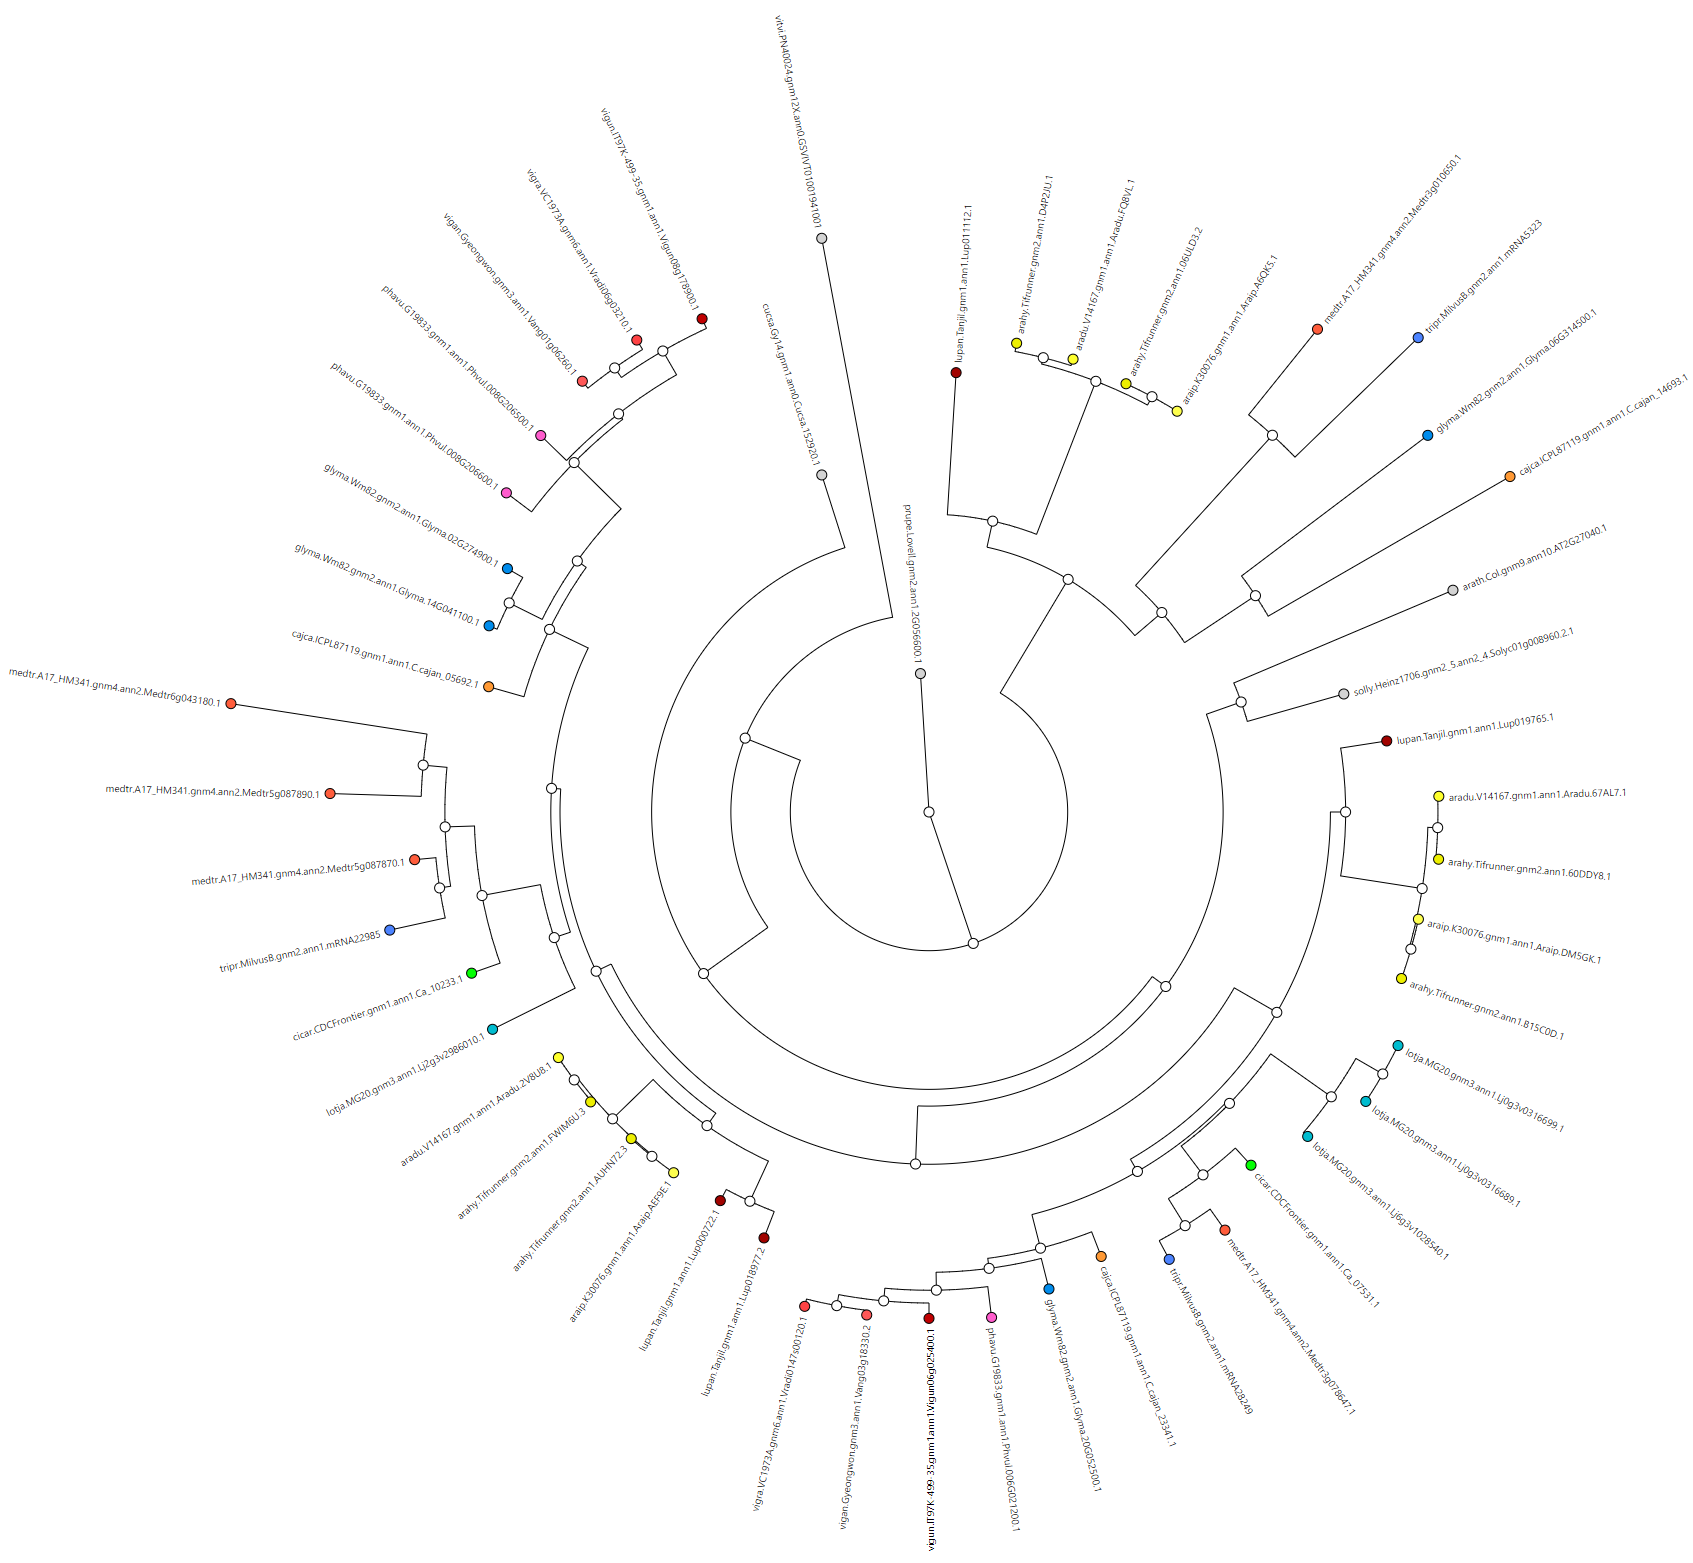
\includegraphics[width=0.55\linewidth]{imgs/radial-color.png}
			    \caption{Phylotree in radial format}
			\end{figure}
		\end{frame}
            \begin{frame}{Results}
		\begin{figure}
			\centering
			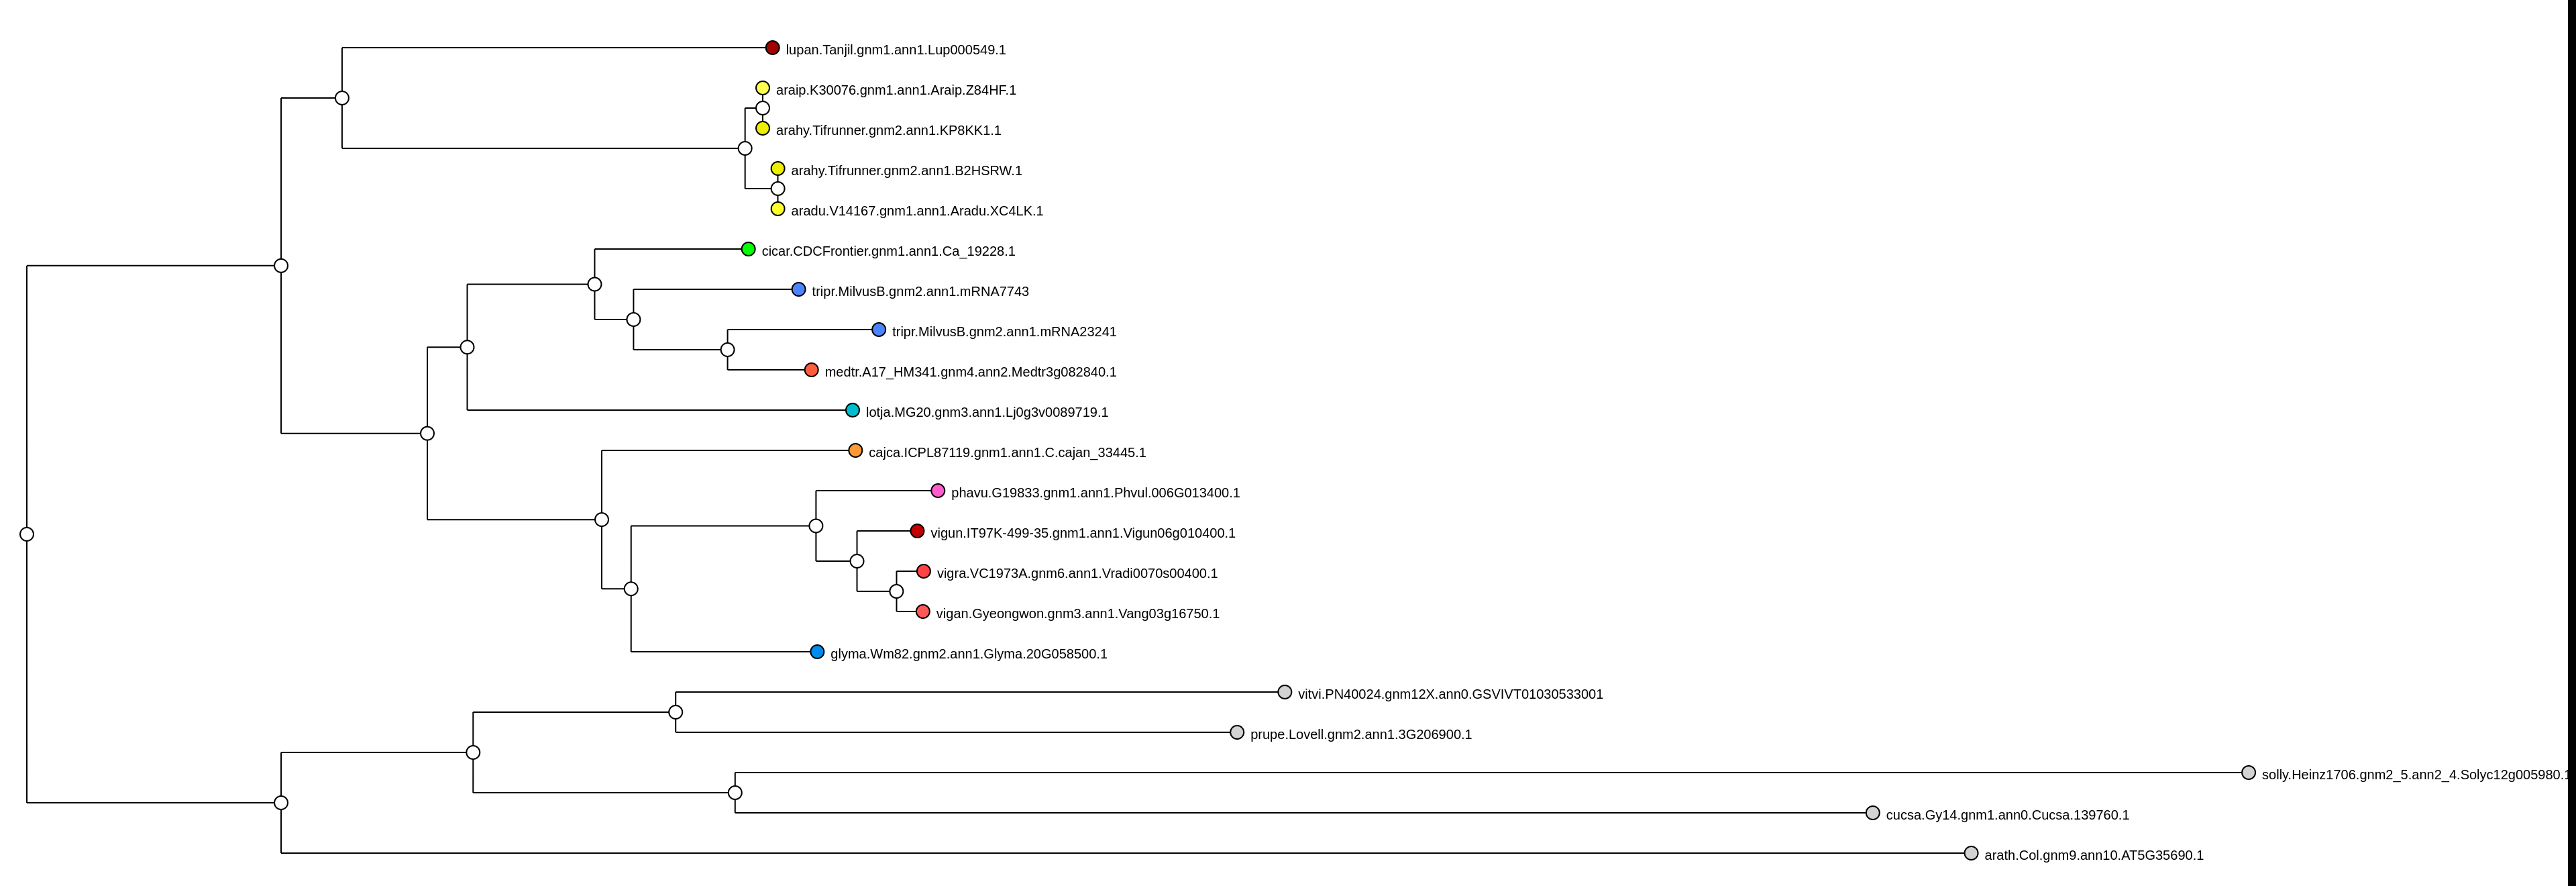
\includegraphics[width=0.6\linewidth]{imgs/vertical-lis-tree.png}
			\caption{Phylotree in vertical format}
		\end{figure}
		\end{frame}
  \begin{frame}
  \large{\bf{So why is this important?}}
  \end{frame}
  \begin{frame}
\large{\bf{{What I learned}}}
  \end{frame}
				\begin{frame}
			\large{\textbf{Questions?}}	
		\end{frame}
		
			

\end{document}
